
% Default to the notebook output style

    


% Inherit from the specified cell style.




    
\documentclass[11pt]{article}

    
    
    \usepackage[T1]{fontenc}
    % Nicer default font (+ math font) than Computer Modern for most use cases
    \usepackage{mathpazo}

    % Basic figure setup, for now with no caption control since it's done
    % automatically by Pandoc (which extracts ![](path) syntax from Markdown).
    \usepackage{graphicx}
    % We will generate all images so they have a width \maxwidth. This means
    % that they will get their normal width if they fit onto the page, but
    % are scaled down if they would overflow the margins.
    \makeatletter
    \def\maxwidth{\ifdim\Gin@nat@width>\linewidth\linewidth
    \else\Gin@nat@width\fi}
    \makeatother
    \let\Oldincludegraphics\includegraphics
    % Set max figure width to be 80% of text width, for now hardcoded.
    \renewcommand{\includegraphics}[1]{\Oldincludegraphics[width=.8\maxwidth]{#1}}
    % Ensure that by default, figures have no caption (until we provide a
    % proper Figure object with a Caption API and a way to capture that
    % in the conversion process - todo).
    \usepackage{caption}
    \DeclareCaptionLabelFormat{nolabel}{}
    \captionsetup{labelformat=nolabel}

    \usepackage{adjustbox} % Used to constrain images to a maximum size 
    \usepackage{xcolor} % Allow colors to be defined
    \usepackage{enumerate} % Needed for markdown enumerations to work
    \usepackage{geometry} % Used to adjust the document margins
    \usepackage{amsmath} % Equations
    \usepackage{amssymb} % Equations
    \usepackage{textcomp} % defines textquotesingle
    % Hack from http://tex.stackexchange.com/a/47451/13684:
    \AtBeginDocument{%
        \def\PYZsq{\textquotesingle}% Upright quotes in Pygmentized code
    }
    \usepackage{upquote} % Upright quotes for verbatim code
    \usepackage{eurosym} % defines \euro
    \usepackage[mathletters]{ucs} % Extended unicode (utf-8) support
    \usepackage[utf8x]{inputenc} % Allow utf-8 characters in the tex document
    \usepackage{fancyvrb} % verbatim replacement that allows latex
    \usepackage{grffile} % extends the file name processing of package graphics 
                         % to support a larger range 
    % The hyperref package gives us a pdf with properly built
    % internal navigation ('pdf bookmarks' for the table of contents,
    % internal cross-reference links, web links for URLs, etc.)
    \usepackage{hyperref}
    \usepackage{longtable} % longtable support required by pandoc >1.10
    \usepackage{booktabs}  % table support for pandoc > 1.12.2
    \usepackage[inline]{enumitem} % IRkernel/repr support (it uses the enumerate* environment)
    \usepackage[normalem]{ulem} % ulem is needed to support strikethroughs (\sout)
                                % normalem makes italics be italics, not underlines
    \usepackage{mathrsfs}
    

    
    
    % Colors for the hyperref package
    \definecolor{urlcolor}{rgb}{0,.145,.698}
    \definecolor{linkcolor}{rgb}{.71,0.21,0.01}
    \definecolor{citecolor}{rgb}{.12,.54,.11}

    % ANSI colors
    \definecolor{ansi-black}{HTML}{3E424D}
    \definecolor{ansi-black-intense}{HTML}{282C36}
    \definecolor{ansi-red}{HTML}{E75C58}
    \definecolor{ansi-red-intense}{HTML}{B22B31}
    \definecolor{ansi-green}{HTML}{00A250}
    \definecolor{ansi-green-intense}{HTML}{007427}
    \definecolor{ansi-yellow}{HTML}{DDB62B}
    \definecolor{ansi-yellow-intense}{HTML}{B27D12}
    \definecolor{ansi-blue}{HTML}{208FFB}
    \definecolor{ansi-blue-intense}{HTML}{0065CA}
    \definecolor{ansi-magenta}{HTML}{D160C4}
    \definecolor{ansi-magenta-intense}{HTML}{A03196}
    \definecolor{ansi-cyan}{HTML}{60C6C8}
    \definecolor{ansi-cyan-intense}{HTML}{258F8F}
    \definecolor{ansi-white}{HTML}{C5C1B4}
    \definecolor{ansi-white-intense}{HTML}{A1A6B2}
    \definecolor{ansi-default-inverse-fg}{HTML}{FFFFFF}
    \definecolor{ansi-default-inverse-bg}{HTML}{000000}

    % commands and environments needed by pandoc snippets
    % extracted from the output of `pandoc -s`
    \providecommand{\tightlist}{%
      \setlength{\itemsep}{0pt}\setlength{\parskip}{0pt}}
    \DefineVerbatimEnvironment{Highlighting}{Verbatim}{commandchars=\\\{\}}
    % Add ',fontsize=\small' for more characters per line
    \newenvironment{Shaded}{}{}
    \newcommand{\KeywordTok}[1]{\textcolor[rgb]{0.00,0.44,0.13}{\textbf{{#1}}}}
    \newcommand{\DataTypeTok}[1]{\textcolor[rgb]{0.56,0.13,0.00}{{#1}}}
    \newcommand{\DecValTok}[1]{\textcolor[rgb]{0.25,0.63,0.44}{{#1}}}
    \newcommand{\BaseNTok}[1]{\textcolor[rgb]{0.25,0.63,0.44}{{#1}}}
    \newcommand{\FloatTok}[1]{\textcolor[rgb]{0.25,0.63,0.44}{{#1}}}
    \newcommand{\CharTok}[1]{\textcolor[rgb]{0.25,0.44,0.63}{{#1}}}
    \newcommand{\StringTok}[1]{\textcolor[rgb]{0.25,0.44,0.63}{{#1}}}
    \newcommand{\CommentTok}[1]{\textcolor[rgb]{0.38,0.63,0.69}{\textit{{#1}}}}
    \newcommand{\OtherTok}[1]{\textcolor[rgb]{0.00,0.44,0.13}{{#1}}}
    \newcommand{\AlertTok}[1]{\textcolor[rgb]{1.00,0.00,0.00}{\textbf{{#1}}}}
    \newcommand{\FunctionTok}[1]{\textcolor[rgb]{0.02,0.16,0.49}{{#1}}}
    \newcommand{\RegionMarkerTok}[1]{{#1}}
    \newcommand{\ErrorTok}[1]{\textcolor[rgb]{1.00,0.00,0.00}{\textbf{{#1}}}}
    \newcommand{\NormalTok}[1]{{#1}}
    
    % Additional commands for more recent versions of Pandoc
    \newcommand{\ConstantTok}[1]{\textcolor[rgb]{0.53,0.00,0.00}{{#1}}}
    \newcommand{\SpecialCharTok}[1]{\textcolor[rgb]{0.25,0.44,0.63}{{#1}}}
    \newcommand{\VerbatimStringTok}[1]{\textcolor[rgb]{0.25,0.44,0.63}{{#1}}}
    \newcommand{\SpecialStringTok}[1]{\textcolor[rgb]{0.73,0.40,0.53}{{#1}}}
    \newcommand{\ImportTok}[1]{{#1}}
    \newcommand{\DocumentationTok}[1]{\textcolor[rgb]{0.73,0.13,0.13}{\textit{{#1}}}}
    \newcommand{\AnnotationTok}[1]{\textcolor[rgb]{0.38,0.63,0.69}{\textbf{\textit{{#1}}}}}
    \newcommand{\CommentVarTok}[1]{\textcolor[rgb]{0.38,0.63,0.69}{\textbf{\textit{{#1}}}}}
    \newcommand{\VariableTok}[1]{\textcolor[rgb]{0.10,0.09,0.49}{{#1}}}
    \newcommand{\ControlFlowTok}[1]{\textcolor[rgb]{0.00,0.44,0.13}{\textbf{{#1}}}}
    \newcommand{\OperatorTok}[1]{\textcolor[rgb]{0.40,0.40,0.40}{{#1}}}
    \newcommand{\BuiltInTok}[1]{{#1}}
    \newcommand{\ExtensionTok}[1]{{#1}}
    \newcommand{\PreprocessorTok}[1]{\textcolor[rgb]{0.74,0.48,0.00}{{#1}}}
    \newcommand{\AttributeTok}[1]{\textcolor[rgb]{0.49,0.56,0.16}{{#1}}}
    \newcommand{\InformationTok}[1]{\textcolor[rgb]{0.38,0.63,0.69}{\textbf{\textit{{#1}}}}}
    \newcommand{\WarningTok}[1]{\textcolor[rgb]{0.38,0.63,0.69}{\textbf{\textit{{#1}}}}}
    
    
    % Define a nice break command that doesn't care if a line doesn't already
    % exist.
    \def\br{\hspace*{\fill} \\* }
    % Math Jax compatibility definitions
    \def\gt{>}
    \def\lt{<}
    \let\Oldtex\TeX
    \let\Oldlatex\LaTeX
    \renewcommand{\TeX}{\textrm{\Oldtex}}
    \renewcommand{\LaTeX}{\textrm{\Oldlatex}}
    % Document parameters
    % Document title
    \title{6. Experimentos Compuestos}
    
    
    
    
    

    % Pygments definitions
    
\makeatletter
\def\PY@reset{\let\PY@it=\relax \let\PY@bf=\relax%
    \let\PY@ul=\relax \let\PY@tc=\relax%
    \let\PY@bc=\relax \let\PY@ff=\relax}
\def\PY@tok#1{\csname PY@tok@#1\endcsname}
\def\PY@toks#1+{\ifx\relax#1\empty\else%
    \PY@tok{#1}\expandafter\PY@toks\fi}
\def\PY@do#1{\PY@bc{\PY@tc{\PY@ul{%
    \PY@it{\PY@bf{\PY@ff{#1}}}}}}}
\def\PY#1#2{\PY@reset\PY@toks#1+\relax+\PY@do{#2}}

\expandafter\def\csname PY@tok@w\endcsname{\def\PY@tc##1{\textcolor[rgb]{0.73,0.73,0.73}{##1}}}
\expandafter\def\csname PY@tok@c\endcsname{\let\PY@it=\textit\def\PY@tc##1{\textcolor[rgb]{0.25,0.50,0.50}{##1}}}
\expandafter\def\csname PY@tok@cp\endcsname{\def\PY@tc##1{\textcolor[rgb]{0.74,0.48,0.00}{##1}}}
\expandafter\def\csname PY@tok@k\endcsname{\let\PY@bf=\textbf\def\PY@tc##1{\textcolor[rgb]{0.00,0.50,0.00}{##1}}}
\expandafter\def\csname PY@tok@kp\endcsname{\def\PY@tc##1{\textcolor[rgb]{0.00,0.50,0.00}{##1}}}
\expandafter\def\csname PY@tok@kt\endcsname{\def\PY@tc##1{\textcolor[rgb]{0.69,0.00,0.25}{##1}}}
\expandafter\def\csname PY@tok@o\endcsname{\def\PY@tc##1{\textcolor[rgb]{0.40,0.40,0.40}{##1}}}
\expandafter\def\csname PY@tok@ow\endcsname{\let\PY@bf=\textbf\def\PY@tc##1{\textcolor[rgb]{0.67,0.13,1.00}{##1}}}
\expandafter\def\csname PY@tok@nb\endcsname{\def\PY@tc##1{\textcolor[rgb]{0.00,0.50,0.00}{##1}}}
\expandafter\def\csname PY@tok@nf\endcsname{\def\PY@tc##1{\textcolor[rgb]{0.00,0.00,1.00}{##1}}}
\expandafter\def\csname PY@tok@nc\endcsname{\let\PY@bf=\textbf\def\PY@tc##1{\textcolor[rgb]{0.00,0.00,1.00}{##1}}}
\expandafter\def\csname PY@tok@nn\endcsname{\let\PY@bf=\textbf\def\PY@tc##1{\textcolor[rgb]{0.00,0.00,1.00}{##1}}}
\expandafter\def\csname PY@tok@ne\endcsname{\let\PY@bf=\textbf\def\PY@tc##1{\textcolor[rgb]{0.82,0.25,0.23}{##1}}}
\expandafter\def\csname PY@tok@nv\endcsname{\def\PY@tc##1{\textcolor[rgb]{0.10,0.09,0.49}{##1}}}
\expandafter\def\csname PY@tok@no\endcsname{\def\PY@tc##1{\textcolor[rgb]{0.53,0.00,0.00}{##1}}}
\expandafter\def\csname PY@tok@nl\endcsname{\def\PY@tc##1{\textcolor[rgb]{0.63,0.63,0.00}{##1}}}
\expandafter\def\csname PY@tok@ni\endcsname{\let\PY@bf=\textbf\def\PY@tc##1{\textcolor[rgb]{0.60,0.60,0.60}{##1}}}
\expandafter\def\csname PY@tok@na\endcsname{\def\PY@tc##1{\textcolor[rgb]{0.49,0.56,0.16}{##1}}}
\expandafter\def\csname PY@tok@nt\endcsname{\let\PY@bf=\textbf\def\PY@tc##1{\textcolor[rgb]{0.00,0.50,0.00}{##1}}}
\expandafter\def\csname PY@tok@nd\endcsname{\def\PY@tc##1{\textcolor[rgb]{0.67,0.13,1.00}{##1}}}
\expandafter\def\csname PY@tok@s\endcsname{\def\PY@tc##1{\textcolor[rgb]{0.73,0.13,0.13}{##1}}}
\expandafter\def\csname PY@tok@sd\endcsname{\let\PY@it=\textit\def\PY@tc##1{\textcolor[rgb]{0.73,0.13,0.13}{##1}}}
\expandafter\def\csname PY@tok@si\endcsname{\let\PY@bf=\textbf\def\PY@tc##1{\textcolor[rgb]{0.73,0.40,0.53}{##1}}}
\expandafter\def\csname PY@tok@se\endcsname{\let\PY@bf=\textbf\def\PY@tc##1{\textcolor[rgb]{0.73,0.40,0.13}{##1}}}
\expandafter\def\csname PY@tok@sr\endcsname{\def\PY@tc##1{\textcolor[rgb]{0.73,0.40,0.53}{##1}}}
\expandafter\def\csname PY@tok@ss\endcsname{\def\PY@tc##1{\textcolor[rgb]{0.10,0.09,0.49}{##1}}}
\expandafter\def\csname PY@tok@sx\endcsname{\def\PY@tc##1{\textcolor[rgb]{0.00,0.50,0.00}{##1}}}
\expandafter\def\csname PY@tok@m\endcsname{\def\PY@tc##1{\textcolor[rgb]{0.40,0.40,0.40}{##1}}}
\expandafter\def\csname PY@tok@gh\endcsname{\let\PY@bf=\textbf\def\PY@tc##1{\textcolor[rgb]{0.00,0.00,0.50}{##1}}}
\expandafter\def\csname PY@tok@gu\endcsname{\let\PY@bf=\textbf\def\PY@tc##1{\textcolor[rgb]{0.50,0.00,0.50}{##1}}}
\expandafter\def\csname PY@tok@gd\endcsname{\def\PY@tc##1{\textcolor[rgb]{0.63,0.00,0.00}{##1}}}
\expandafter\def\csname PY@tok@gi\endcsname{\def\PY@tc##1{\textcolor[rgb]{0.00,0.63,0.00}{##1}}}
\expandafter\def\csname PY@tok@gr\endcsname{\def\PY@tc##1{\textcolor[rgb]{1.00,0.00,0.00}{##1}}}
\expandafter\def\csname PY@tok@ge\endcsname{\let\PY@it=\textit}
\expandafter\def\csname PY@tok@gs\endcsname{\let\PY@bf=\textbf}
\expandafter\def\csname PY@tok@gp\endcsname{\let\PY@bf=\textbf\def\PY@tc##1{\textcolor[rgb]{0.00,0.00,0.50}{##1}}}
\expandafter\def\csname PY@tok@go\endcsname{\def\PY@tc##1{\textcolor[rgb]{0.53,0.53,0.53}{##1}}}
\expandafter\def\csname PY@tok@gt\endcsname{\def\PY@tc##1{\textcolor[rgb]{0.00,0.27,0.87}{##1}}}
\expandafter\def\csname PY@tok@err\endcsname{\def\PY@bc##1{\setlength{\fboxsep}{0pt}\fcolorbox[rgb]{1.00,0.00,0.00}{1,1,1}{\strut ##1}}}
\expandafter\def\csname PY@tok@kc\endcsname{\let\PY@bf=\textbf\def\PY@tc##1{\textcolor[rgb]{0.00,0.50,0.00}{##1}}}
\expandafter\def\csname PY@tok@kd\endcsname{\let\PY@bf=\textbf\def\PY@tc##1{\textcolor[rgb]{0.00,0.50,0.00}{##1}}}
\expandafter\def\csname PY@tok@kn\endcsname{\let\PY@bf=\textbf\def\PY@tc##1{\textcolor[rgb]{0.00,0.50,0.00}{##1}}}
\expandafter\def\csname PY@tok@kr\endcsname{\let\PY@bf=\textbf\def\PY@tc##1{\textcolor[rgb]{0.00,0.50,0.00}{##1}}}
\expandafter\def\csname PY@tok@bp\endcsname{\def\PY@tc##1{\textcolor[rgb]{0.00,0.50,0.00}{##1}}}
\expandafter\def\csname PY@tok@fm\endcsname{\def\PY@tc##1{\textcolor[rgb]{0.00,0.00,1.00}{##1}}}
\expandafter\def\csname PY@tok@vc\endcsname{\def\PY@tc##1{\textcolor[rgb]{0.10,0.09,0.49}{##1}}}
\expandafter\def\csname PY@tok@vg\endcsname{\def\PY@tc##1{\textcolor[rgb]{0.10,0.09,0.49}{##1}}}
\expandafter\def\csname PY@tok@vi\endcsname{\def\PY@tc##1{\textcolor[rgb]{0.10,0.09,0.49}{##1}}}
\expandafter\def\csname PY@tok@vm\endcsname{\def\PY@tc##1{\textcolor[rgb]{0.10,0.09,0.49}{##1}}}
\expandafter\def\csname PY@tok@sa\endcsname{\def\PY@tc##1{\textcolor[rgb]{0.73,0.13,0.13}{##1}}}
\expandafter\def\csname PY@tok@sb\endcsname{\def\PY@tc##1{\textcolor[rgb]{0.73,0.13,0.13}{##1}}}
\expandafter\def\csname PY@tok@sc\endcsname{\def\PY@tc##1{\textcolor[rgb]{0.73,0.13,0.13}{##1}}}
\expandafter\def\csname PY@tok@dl\endcsname{\def\PY@tc##1{\textcolor[rgb]{0.73,0.13,0.13}{##1}}}
\expandafter\def\csname PY@tok@s2\endcsname{\def\PY@tc##1{\textcolor[rgb]{0.73,0.13,0.13}{##1}}}
\expandafter\def\csname PY@tok@sh\endcsname{\def\PY@tc##1{\textcolor[rgb]{0.73,0.13,0.13}{##1}}}
\expandafter\def\csname PY@tok@s1\endcsname{\def\PY@tc##1{\textcolor[rgb]{0.73,0.13,0.13}{##1}}}
\expandafter\def\csname PY@tok@mb\endcsname{\def\PY@tc##1{\textcolor[rgb]{0.40,0.40,0.40}{##1}}}
\expandafter\def\csname PY@tok@mf\endcsname{\def\PY@tc##1{\textcolor[rgb]{0.40,0.40,0.40}{##1}}}
\expandafter\def\csname PY@tok@mh\endcsname{\def\PY@tc##1{\textcolor[rgb]{0.40,0.40,0.40}{##1}}}
\expandafter\def\csname PY@tok@mi\endcsname{\def\PY@tc##1{\textcolor[rgb]{0.40,0.40,0.40}{##1}}}
\expandafter\def\csname PY@tok@il\endcsname{\def\PY@tc##1{\textcolor[rgb]{0.40,0.40,0.40}{##1}}}
\expandafter\def\csname PY@tok@mo\endcsname{\def\PY@tc##1{\textcolor[rgb]{0.40,0.40,0.40}{##1}}}
\expandafter\def\csname PY@tok@ch\endcsname{\let\PY@it=\textit\def\PY@tc##1{\textcolor[rgb]{0.25,0.50,0.50}{##1}}}
\expandafter\def\csname PY@tok@cm\endcsname{\let\PY@it=\textit\def\PY@tc##1{\textcolor[rgb]{0.25,0.50,0.50}{##1}}}
\expandafter\def\csname PY@tok@cpf\endcsname{\let\PY@it=\textit\def\PY@tc##1{\textcolor[rgb]{0.25,0.50,0.50}{##1}}}
\expandafter\def\csname PY@tok@c1\endcsname{\let\PY@it=\textit\def\PY@tc##1{\textcolor[rgb]{0.25,0.50,0.50}{##1}}}
\expandafter\def\csname PY@tok@cs\endcsname{\let\PY@it=\textit\def\PY@tc##1{\textcolor[rgb]{0.25,0.50,0.50}{##1}}}

\def\PYZbs{\char`\\}
\def\PYZus{\char`\_}
\def\PYZob{\char`\{}
\def\PYZcb{\char`\}}
\def\PYZca{\char`\^}
\def\PYZam{\char`\&}
\def\PYZlt{\char`\<}
\def\PYZgt{\char`\>}
\def\PYZsh{\char`\#}
\def\PYZpc{\char`\%}
\def\PYZdl{\char`\$}
\def\PYZhy{\char`\-}
\def\PYZsq{\char`\'}
\def\PYZdq{\char`\"}
\def\PYZti{\char`\~}
% for compatibility with earlier versions
\def\PYZat{@}
\def\PYZlb{[}
\def\PYZrb{]}
\makeatother


    % Exact colors from NB
    \definecolor{incolor}{rgb}{0.0, 0.0, 0.5}
    \definecolor{outcolor}{rgb}{0.545, 0.0, 0.0}



    
    % Prevent overflowing lines due to hard-to-break entities
    \sloppy 
    % Setup hyperref package
    \hypersetup{
      breaklinks=true,  % so long urls are correctly broken across lines
      colorlinks=true,
      urlcolor=urlcolor,
      linkcolor=linkcolor,
      citecolor=citecolor,
      }
    % Slightly bigger margins than the latex defaults
    
    \geometry{verbose,tmargin=1in,bmargin=1in,lmargin=1in,rmargin=1in}
    
    

    \begin{document}
    
    
    \maketitle
    
    

    
    \section*{6. Experimentos Compuestos. Pruebas de
Bernoulli}\label{experimentos-compuestos.-pruebas-de-bernoulli}

\subsection*{Experimentos Compuestos}\label{experimentos-compuestos}

Con frecuencia estamos interesados en experimentos aleatorios que
acontecen simultánea o sucesivamente. Tales experimentos se modelan con
sus propios \textbf{espacios de probabilidad marginales}, pero al
interesarnos la relación entre ellos es necesario también modelar su
\textbf{espacio de probabilidad conjunto}.

En algunos casos, \textbf{no existe depencia probabilística entre los
experimentos marginales}. En tal caso, \textbf{puede obtenerse
fácilmente la caracterización conjunta a partir de las marginales}. Es
el caso, por ejemplo, en el que lanzamos simultáneamente varios dados, o
en elque lanzamos sucesivamente varias veces la misma moneda.

En otros, \textbf{sí existe dependencia probabilística entre los
experimentos marginales}, en cuyo caso \textbf{se necesita conocer la
caracterización conjunta, que no es posible obtener a partir de las
marginales}. Por ejemplo, un espacio de probabilidad puede modelar que
una persona tenga una enfermedad y otro el resultado de un test
diagnóstico.

    Consideremos que realizamos los experimentos \(\epsilon_1\): "lanzar una
moneda" y \(\epsilon_2\): "lanzar un dado". Tanto el dado como la moneda
son buenos (no están trucados). Ambos experimentos inducen sendos
espacios de probabilidad:

\begin{itemize}
\tightlist
\item
  \(\epsilon_1 (\Omega_1, \mathscr{F}_1, P_1)\), donde:
\begin{itemize}
\item
  \(\Omega_2=\{c,x\}\),
\item
  \(\mathscr{F}_1\) es el conjunto con los \(2^2=4\) sucesos posibles, y
\item
  \(P_1(c)=P_2(x)= \ ^1/_2\)
\end{itemize}
\item
  \(\epsilon_2 (\Omega_2, \mathscr{F}_2, P_2)\), donde:
\begin{itemize}
\item
  \(\Omega_2=\{1,2,3,4,5,6\}\),
\item
  \(\mathscr{F}_2\) es el conjunto con los \(2^6=64\) sucesos posibles,
  y
\item
  \(P_2(1)=P_1(2)=\ldots =P(6)= \ ^1/_6\)
\end{itemize}
\end{itemize}

    El espacio muestral compuesto se obtiene mediante el \textbf{producto
cartesiano} \(\Omega_1 \times \Omega_2\) de los espacios muestrales
marginales, \(\Omega_1\) y \(\Omega_2\), esto es, el conjunto formado
por todos los \textbf{pares ordenados} que podemos obtener a partir de
los elementos de ambos:

\begin{align*}
\Omega_1 \times \Omega_2 = \{&(c,1), (c,2), (c,3), (c,4), (c,5), (c,6),\\ &(x,1), (x,2), (x,3), (x,4), (x,5), (x,6)\}
\end{align*}

\[
\begin{array}{c|cccccccc|c}
  \Omega_1 \times \Omega_2 & 1 & 2 & 3 & 4 & 5 & 6 & \\ 
  \hline
  c & (c,1) & (c,2) & (c,3) & (c,4) & (c,5) & (c,6) &  \\
  \hline
  x & (c,1) & (c,2) & (c,3) & (c,4) & (c,5) & (c,6) & 
 \end{array}
\]

    Sobre el espacio muestral conjunto puede definirse un álgebra de
sucesos, consistente en todos los subconjuntos que puedan formarse a
partir del mismo (en general, con ciertas restricciones que ahora no nos
preocupan). Este álgebra de sucesos puede obtenerse con el producto
cartesiano de las álgebras de sucesos de los espacios de probabilidad
marginales, \(\mathscr{F}_1\times \mathscr{F}_2\).

En nuestro caso, tenemos \(2⁶= 64\) sucesos en cada espacio muestral,
por lo que habrá \(2^12=1024\) sucesos en el espacio de probabilidad
conjunto. Algunos sucesos relevantes son: 
\begin{itemize}
\item Suceso imposible:
\(\emptyset = \{(A_1,\emptyset),(\emptyset,A_2),(\emptyset,\emptyset)\}\)
\item Suceso seguro: \(\Omega_1 \times \Omega_2\) 
\item Suceso marginal \(A_1\)
en primer experimento: \(A_1 \times \Omega_2\) 
\item Suceso marginal \(A_2\)
en segundo experimento: \(\Omega_1 \times A_2\) 
\item Suceso
\(A_1 \times A_2 = (A_1 \times \Omega_2) \bigcap (\Omega_1 \times A_2)\)
\end{itemize}

    Seguidamente, asignamos probabilidades a los elementos del espacio
muestral conjunto.

\[
\begin{array}{c|cccccccc|c}
  P & 1 & 2 & 3 & 4 & 5 & 6 & \\ 
  \hline
  c & P(c,1) & P(c,2) & P(c,3) & P(c,4) & P(c,5) & P(c,6) &  \\
  \hline
  x & P(c,1) & P(c,2) & P(c,3) & P(c,4) & P(c,5) & P(c,6) & 
 \end{array}
\]

Y, con ello, es posible asignar probabilidades a los sucesos de
\(\mathscr{F}_1\times \mathscr{F}_2\): 
\begin{itemize}
\item Suceso imposible:
\(P(A_1,\emptyset)=P(\emptyset,A_2)=P(\emptyset,\emptyset)=0\) 
\item Suceso
seguro: \(P(\Omega_1 \times \Omega_2)=1\). La suma de probabilidades es
1. 
\item Cálculos de probabilidades marginales a partir de probabilidades
conjuntas: 
\begin{itemize}
\item \(P_1(A_1)=P(A_1 \times \Omega_2)\) 
\item \(P_2(A_2)=P(\Omega_1 \times A_2)\) 
\item
\(P(A_1 \times A_2) = P((A_1 \times \Omega_2) \bigcap (\Omega_1 \times A_2))\)
\end{itemize}
\item En general, no puede calcularse la probabilidad conjunta a partir de
las probabilidades marginales.
\end{itemize}

    Por tanto, es posible definir un experimento de probabilidad compuesto,
cuyo espacio de probabilidad conjunto se modela a partir de los
marginales:

\[\epsilon_1 \times \epsilon_2 =\{\Omega_1 \times \Omega_2, \mathscr{F}_1\times \mathscr{F}_2, P \}\]

Las probabilidades conjuntas, en general, no están determinadas por las
marginales:

\[P(A_1 \times A_2) = P((A_1 \times \Omega_2) \bigcap (\Omega_1 \times A_2))\]

Sin embargo, considerando que dos experimentos son independientes si y
sólo si lo son todos sus sucesos, \textbf{en caso de independencia es
posible calcular las probabilidades conjuntas a partir de las
marginales}:

\[P(A_1 \times A_2) = P((A_1 \times \Omega_2)) P((\Omega_1 \times A_2))= P_1(A_1)P_2(A_2)\]

    En el caso de nuestro ejemplo de experimento compuesto, consideremos el
suceso \((c,3)\):

\[P(\{c\}\times \Omega_2)= P_1(c) =\ ^1/_2 \qquad P(\Omega_1 \times \{3\}) = P_2(3)=\ ^1/_6\]

Y las probabilidades de elementos arbitrarios del espacio muestral:

\[P((c,3))= P((\{c\}\times\Omega_2) \bigcap (\Omega_1 \times \{3\}))\]

En este experimento compuesto \textbf{podemos asumir independencia}, por
tanto:

\[P((c,3)) = P(\{c\}\times \Omega_2) P(\Omega_1\times\{3\})=P_1(c)P_2(3)=\frac{1}{2}\frac{1}{6}=\frac{1}{12}\]

    Reptiendo el cálculo visto para todos los eleemntos del espacio muestral
conjunto, podemos hacer la asignación de probabilidades:

\[
\begin{array}{c|cccccccc|c}
  P & 1 & 2 & 3 & 4 & 5 & 6 & \\ 
  \hline
  c & P(c,1) = \ ^1/_{12} & P(c,2) = \ ^1/_{12} & P(c,3) = \ ^1/_{12} & P(c,4) = \ ^1/_{12} & P(c,5) = \ ^1/_{12} & P(c,6) = \ ^1/_{12} &  \\
  \hline
  x & P(c,1) = \ ^1/_{12} & P(c,2) = \ ^1/_{12} & P(c,3) = \ ^1/_{12} & P(c,4) = \ ^1/_{12} & P(c,5) = \ ^1/_{12} & P(c,6) = \ ^1/_{12} & 
 \end{array}
\]

Puede advertirse fácilmente que la suma de todas las probabilidades es
\(1\), como corresponde al suceso seguro.

    \subsubsection*{Pruebas repetidas de
Bernoulli}\label{pruebas-repetidas-de-bernoulli}

Podemos pensar en experimentos compuestos por más de dos experimentos
marginales. Un caso habitual es cuando se repite de forma
\textbf{independiente} \(N\) veces un mismo experimento

\[\epsilon \times \ldots \times \epsilon (\Omega \times\ldots \Omega, \mathscr{F}\times \ldots \times \mathscr{F}, P)\]

En este caso, podemos fácilmente asignar probabilidades:

\[P(A_1 \times \ldots A_N) = P(A_1)\ldots P(A_N)\]

Un caso habitual es de repetir \textbf{experimentos de Bernoulli}. Se
trata de experimentos con dos resultados posibles, acertar o fallar, en
lo que \(P(acertar)=p\) y \(P(fallar)=1-p\).

    Por ejemplo, en el lanzamiento de una moneda trucada la probabilidad de
sacar cara (acertar, en este caso) es \(P(cara)=p\).

Si repetimos \(N\) veces el experimento, ¿cuál será la probabilidad de
acertar \(n\) veces?

Supongamos el siguiente suceso \(A\), correspondiente a una secuencia de
\(N=10\) lanzamientos:

\[A=(c,c,x,x,x,c,c,x,c, c)\]

Es fácil ver que \[P(A)=p^6(1-p)^4\]

    Cualquier secuencia que contenga \(6\) caras y \(4\) cruces tendrá
idéntica probabilidad. En ocasiones, no nos interesa el orden en el que
han salido los resultados, sino el número total de los mismos. Por
ejemplo, nos interesa saber cuál es la probabilidad de que al lanzar
\(N=10\) veces la moneda tengamos \(n=6\) caras (aciertos). En tales
casos, es necesario calcular el número de combinaciones que podemos
obtener de \(N\) elementos agrupados de \(n\) en \(n\):

\[\binom{N}{n} = \frac{N!}{n!(N-n)!} \qquad \binom{10}{6} = \frac{10!}{6!(10-6)!}=210\]

Por lo que la probabilidad de \(6\) aciertos o caras será
\(210 p^6(1-p)^4\). En general, la probabilidad P(n; N) de \(n\)
aciertos en \(N\) intentos es:

\[P(n;N) = \binom{N}{n}p^n(1-p)^{N-n}\]

    \section*{Parametrización de espacios de
probabilidad}\label{parametrizaciuxf3n-de-espacios-de-probabilidad}

Es frecuente que un espacio de probabilidad tenga sus probabilidades
parametrizadas por un hecho o experimento externo al mismo.

Supongamos, por ejemplo, un test diagnóstico de cierta enfermedad. El
test admite dos resultados posibles: 
\begin{itemize}
\item \(T^+\) = "el test resulta
positivo" y 
\item \(T^-\) = "el test resulta negativo",
\end{itemize}

Sin embargo, el resultado del test está íntimamente relacionado con la
salud de la persona a la que se le aplica: 
\begin{itemize}
\item \(S_E\) = "SI tiene la
enfermedad" y 
\item \(N_E\) = "NO tiene la enfermedad".
\end{itemize}

    El resultado del test se modela mediante un espacio de probabilidad.
Ciertamente, el test puede fallar y resultar positivo cuando la persona
está sana, o negativo cuando está enferma. Esto justifica que se modele
probabilísticamente.

Sin embargo, es evidente que el modelado probabilístico debe tener en
consideración si la persona a la que se le aplica el test está sana o
enferma. De otro modo, el test sería inútil. Esperamos que el test de
positivo cuando la persona esté enferma y negativo cuando está sana, y
no al revés, sin perjuicio de que pueda equivocarse a veces.

Este razonamiento es propio de situaciones en las que existen
\textbf{relaciones de causalidad que no son deterministas}: la
enfermedad o ausencia de la misma es \textbf{causa del efecto
observable} consistente en tener un resultado positivo o negatrivo en el
test, pero el test puede fallar por lo que la relación no es
determinista.

    Esta preocupación se extiende a una infinidad de situaciones diferentes
en múltiples campos muy distantes entre sí. Pensemos en un RADAR, que es
un sistema diseñado para la detección y seguimiento de blancos, con
distintas aplicaciones tanto civiles como militares. Un suceso que
podemos medir es que el RADAR detecta un blanco, y queremos estar
seguros de que realmente hay un blanco y de que no se trata de una
\emph{falsa alarma}. Otro suceso que podemos medir es que el RADAR no
detecta nada, pero nuestro interés está en que realmente no haya blanco
y no se haya producido una \emph{pérdida}.

Otro ejemplo es el de un sistema de comunicación digital, que en cada
instante transmite uno entre \(N\) símbolos posibles que tiene en su
alfabeto. Sin embargo, al codificarlo en un señal electromagnética que,
en su propagación, se ve afectada por distorsión y atenuación del canal,
intereferencias y ruido, pueden producirse errores en la detección. En
este caso, los sucesos que podemos medir son los símbolos que recupera
el receptor, mientras que los sucesos relacionados en los que estamos
interesados son los símbolos que realmente ha transmitido el emisor.

    \subsection*{Estrategia clásica versus
bayesiana}\label{estrategia-cluxe1sica-versus-bayesiana}

Al modelar la relación del espacio de probabilidad observable con la
causa subyacente, podemos considerar: 
\begin{itemize}
\item \textbf{Estrategia clásica}: Que
la causa es un parámetro determinista. Las verosimilitudes de las causas
resultan de las probabilidades de las observaciones parametrizadas por
las causas posibles: 
\begin{itemize}
\item \(L(S_E)=P(T^+; S_E)=1-P(T^-; S_E)\) 
\item \(L(N_E)=P(T^-; N_E) = 1-P(T^+; N_E)\) 
\end{itemize}
\item \textbf{Estrategia bayesiana}:
Que la causa es, a su vez, modelable como un experimento aleatorio, en
cuyo caso estaremos ante un experimento compuesto. Ahora \textbf{las
versosimilitudes resultan de las probabilidades condicionadas de la
observación por las causas}. Las probabilidades marginales corresponden
a las probabilidades marginales de las causas, y \textbf{podemos
calcular las probabilidades \emph{a posteriori} de las causas, vistas
las observaciones}, con el Teorema de Bayes. 
\begin{itemize}
\item \(L(S_E)=P(T^+/ S_E)=1-P(T^-/ S_E)\) 
\item \(L(N_E)=P(T^-/ N_E) = 1-P(T^+/ N_E)\)
\end{itemize}
\end{itemize}

    Un caso de especial interés es aquel en el que solo hay \textbf{dos
causas posibles} que identificamos como \textbf{hipótesis} a determinar
a partir de las \textbf{observaciones}. Algunos ejemplos sencillos son 
\begin{itemize}
\item
El test de enfermedad, en el que tenemos dos posibles causas, \(S_E\)
(hay enfermedad) y \(N_E\) (no hay enfermedad), y dos posibles efectos,
\(T⁺\) (test positivo) y \(T^-\) (test negativo). 

Otros equivalentes
son: 
\item La detección RADAR, donde las causas son "hay blanco" y "no hay
blanco" y los efectos "blanco detectado" y "blanco no detectado". 
\item Un
sistema de comunicación digital, en el que las causas son \(0_T\) (se
transmite \(0\)) y \(1_T\) (se transmite \(1\)) y los efectos son
\(0_D\) (se detecta \(0\) en el receptor) y \(1_D\) (se detecta \(1\) en
el receptor) 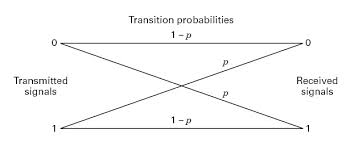
\includegraphics{diagrama_canal_binario.jpg}
\end{itemize}

    Las hipótesis se refieren a las causas de las observaciones. Nuestra
incertidumbre sobre las mismas puede modelarse como parámetros
deterministas desponocidos o como sucesos aleatorios: 
\begin{itemize}
\item \textbf{Hipótesis nula}, \(\mathbf{H_0}\), se refiere al hecho o suceso
de, por ejemplo, no existir enfermedad, blanco o nivel. 
\item \textbf{Hipótesis alternativa}, \(\mathbf{H_1}\), corresponde a la
situación complementaria.
\end{itemize}

Las observaciones mantienen una relación probabilística con las causas,
bien en forma de verosimilitudes parametrizadas por las mismas, bien en
forma de probabilidades condicionadas. Las hipótesis se seleccionan a
partir de las observaciones, considerando su relación con las causas.
Las observaciones son aleatorias, por lo que no determinan con certeza
las causas: 
\begin{itemize}
\item \textbf{Observación nula}, \(\mathbf{O_0}\), aparentemente
la observación respalda la hipótesis nula, por ejemplo, un test negativo
lleva a presumir que no hay enfermedad, o una ausencia de señal RADAR
que no hay blanco. 
\item \textbf{Observación alternativa}, \(\mathbf{O_1}\),
aparentemente a observación respalda la hipótesis alternativa.
\end{itemize}
  
    En el \textbf{esquema clásico}, la elección de la hipótesis se hace
dependiendo de qué verosimilitud sea mayor para una observación dada:

\begin{itemize}
\tightlist
\item
  Se observa \(\mathbf{O_0}\)
\item
  \(L(H_0) = P(O_0;H_0) > L(H_1) = P(O_0;H_1) \implies H_0\).
  Lógicamente el test se diseña para que así sea.
\item
  \(L(H_1) = P(O_0;H_1) > L(H_0) = P(O_0;H_0) \implies H_1\)
\item
  Se observa \(\mathbf{O_1}\)
\item
  \(L(H_1) = P(O_1;H_1) > L(H_0) = P(O_1;H_0) \implies H_1\).
  Lógicamente el test se diseña para que así sea.
\item
  \(L(H_0) = P(O_1;H_0) > L(H_1) = P(O_1;H_1) \implies H_0\).
\end{itemize}

    Las posibles transiciones y sus probabilidades asociadas, parametrizadas
por las hipótesis, son: 
\begin{itemize}
\item \(P(O_0;H_0)\), que corresponde a la
probabilidad de aceptar correctamente la hipótesis nula, de rechazar la
alternativa (no hay blanco, o enfermedad,...) de detectar correctamente
el \(0\), o \textbf{nivel de confianza}. A veces se llama
\textbf{especificidad}. 
\item \(P(O_1;H_1)\), que corresponde a la
probabilidad de rechazar correctamente la hipótesis nula, de aceptar la
alternativa (hay blanco, o enfermedad,...) de detectar correctamente el
\(1\), o \textbf{potencia del test}. También se llama
\textbf{probabilidad de detección}, \(P_D\), o \textbf{sensibilidad}.
\item \(P(O_1;H_0)\equiv\alpha\), que corresponde a la probabilidad de
rechazar erróneamente la hipótesis nula, aceptar erróneamente la
hipótesis alternativa, falso positivo, o \textbf{nivel de
significación}, \(\alpha\), \textbf{probabilidad de error de tipo I},
\(P_{\epsilon_1}\), a veces llamada \textbf{probabilidad de falsa
alarma}, \(P_{FA}\). 
\item \(P(O_0;H_1)\equiv\beta\), que corresponde a la
probabilidad de aceptar erróneamente la hipòtesis nula, rechazar
erróneamente la hipótesis alternativa, falso negativo o
\textbf{probabilidad de error de tipo II}, \(P_{\epsilon_2}\), a veces
llamada \textbf{probabilidad de pérdida}, \(P_{M}\).
\end{itemize}

    Dado que sólo hay dos hipótesis posibles, es fácil advertir que: 
\begin{itemize}
\item \(P(O_1;H_0)\equiv\alpha = 1- P(O_0;H_0) \implies P(H_0;H_0)=1-\alpha\)
\item \(P(O_0;H_1)\equiv\beta = 1- P(O_1;H_1) \implies P(H_1;H_1)=1-\beta\)
\end{itemize}

Los \textbf{tests o contrastes de hipótesis} suelen diseñarse de modo
que: 
\begin{itemize}
\item La potencia \(1-\beta\) sea máxima, esto es, que sea máxima la
sensibilidad o probabilidad de detección. 
\item Que el nivel de
significación \(\alpha\) se mantenga por debajo de un umbral o,
equivalentemente, que la especificidad o nivel de confianza se mantengan
suficientemente altos.
\end{itemize}

    Veamos un primer ejemplo práctico. Supongamos que un sistema RADAR se
diseña con las siguientes características: 
\begin{itemize}
\item Probabilidad de detección:
\(P_D=0.99\) 
\item Probabilidad de falsa alarma: \(P_{FA}\equiv\alpha=0.15\)
\end{itemize}

La hipótesis nula, \(\mathbf{H_0}\), es la ausencia de blanco y la
hipótesis alternativa, \(\mathbf{H_1}\), es la presencia del mismo.

¿Cuáles son su probabilidades de transición? 
\begin{itemize}
\item
\(P(O_1;H_1) = P_D = 1-\beta= 0.99\), que corresponde a la
\textbf{sensibilidad} o \textbf{potencia} del test. 
\item
\(P(O_1;H_0)\equiv\alpha = P_{FA} = 0.15\), que corresponde al
\textbf{nivel de significación} del test o probabilidad de error de tipo
I. 
\item
\(P(O_0;H_1)\equiv\beta = 1-P_D = 0.01\), que es la probabilidad de
pérdida y corresponde a la probabilidad de error de tipo II. 
\item
\(P(O_0;H_0)=1-\alpha = 1-P_{FA} = 0.85\), que corresponde al
\textbf{nivel de confianza} o \textbf{especificidad} del test.
\end{itemize}

    A modo de segundo ejemplo, consideremos un test clínico con las
siguientes características:

\begin{itemize}
\tightlist
\item
  \(\mathbf{H_0}\): no hay enfermedad
\item
  \(\mathbf{H_1}\): hay enfermedad
\item
  Sensibilidad \(1-\beta = 99\%\)
\item
  Especificidad: \(1-\alpha=85\%\)
\end{itemize}

¿Cómo resultan ahora las probabilidades del test?
\begin{itemize}
\item \(P(O_0;H_0)=1-\alpha=0.85\) * \(P(O_1;H_1)=1-\beta=0.99\)
\item \(P(O_1;H_0)\equiv\alpha=0.15\) * \(P(O_0;H_1\equiv\beta=0.01)\)
\end{itemize}

    En el \textbf{esquema bayesiano}, se dispone de las probabilidades
\emph{a priori} de las hipótesis, \(P(H_0)\) y \(P(H_1)\) y de las
probabilidades de transición condionadas, o verosimilitudes: 
\begin{itemize}
\item \(L(H_0) = P(O_0/H_0) = 1-P(O_1/H_0)\),
\item \(L(H_1) = P(O_1/H_1) = 1-P(O_0/H_1)\)
\end{itemize}

La \textbf{probabilidad total} de cada observación es:

\[P(O_0)=P(O_0/H_0)P(H_0)+P(O_0/H_1)P(H_1)\\
P(O_1)=P(O_1/H_0)P(H_0)+P(O_1/H_1)P(H_1)\]

    Las probabilidades \emph{a posteri} resultan:

\begin{itemize}
\tightlist
\item
  Probabilidades de acierto:
  \[P(H_0/O_0)=\frac{P(O_0/H_0)P(H_0)}{P(O_0)}\\
  P(H_1/O_1)=\frac{P(O_1/H_1)P(H_1)}{P(O_1)}\]
\item
  Probabilidad total de acierto:
  \[P(A)=P(H_0/O_0)P(O_0)+P(H_1/O_1)P(O_1)\]
\end{itemize}

    \begin{itemize}
\tightlist
\item
  Probabilidades de error:
  \[P(H_1/O_0)=\frac{P(O_0/H_1)P(H_1)}{P(O_0)}\\
  P(H_0/O_1)=\frac{P(O_1/H_0)P(H_0)}{P(O_1)}\]
\item
  Probabilidad total de error:
  \[P(E)=P(H_1/O_0)P(O_0)+P(H_0/O_1)P(O_1)\]
\end{itemize}

    Podemos extender el número de hipótesis a un número \(K>2\). Esto
resultará de utilidad en problemas de clasificación:

Las hipótesis \(\mathbf{H_0} \ldots \mathbf{H_{K-1}}\) corresponden a
cada una de las clases (o causas) que subyacen como sucesos
condicionantes, o que medimos.

Las probabilidades de transición son
\begin{itemize}
\item
\(P(O_0/H_0), P(O_1/H_0),\ldots P(O_{K-1}/H_0)\) 
\item  ........ 
\item
\(P(O_0/H_{K-1}), P(O_1/H_{K-1}),\ldots P(O_{K-1}/O_{K-1})\)
\end{itemize}

donde: 
\begin{itemize}
\item \(P(O_i/H_i), i=0\ldots K-1\) representan probabilidades de
clasificación correcta. 
\item \(P(O_i/H_j), i\neq j\) representan
probabilidades de error.
\end{itemize}

    % Add a bibliography block to the postdoc
    
    
    
    \end{document}
